\chapter{Introduction}

The success of modern particle physics has been a great success in describing the basic constituents of matter and the fundamental interactions between them.
The Standard Model (SM) of particle physics summarizes the behavior of all observed elementary particles, shown in Figure~\ref{fig:SM_table}.
There are 12 types of elementary fermions, 4 types of elementary gauge bosons, and 1 Higgs boson.
Elementary fermions are matter particles and are further categorized into quarks and leptons.
Both quarks and leptons have 3 generations.
In each generation, there is a charge = $+\frac{2}{3}$ quark (u, c, and \Pqt quarks),
a charge = $-\frac{1}{3}$ quark (d, s, and \Pqb quarks), 
a charge = -1 lepton ($e$, \mu, and \tau ~leptons),
and a neutral lepton ($\nu_{e}$, $\nu_{\mu}$, and $\nu_{\tau}$ neutrinos).
Gauge bosons have spin~=~1 are carriers of fundamental interactions: 
gluons for the strong interaction, photons for the electromagnetic interaction,
and \PW and \PZ bosons for the weak interaction.
Gravity is another fundamental interaction whose quantization has not been observed experimentally,
and is not included in the SM.
The Higgs boson is the only scalar boson (spin~=~0) in the SM.
It plays a special role in the SM as it interacts with all massive elementary particles 
and introduces the mechanism for them to have nonzero masses.
Each of the particles has a counterpart called an antiparticle which has the same mass and spin as the particle itself, 
but opposite charge and other quantum numbers.
The antiparticles of neutral bosons (gluons, photons, \PZ, and Higgs bosons) are themselves.

\begin{figure*}[!htb]
    \centering
    \captionsetup{justification=justified}
    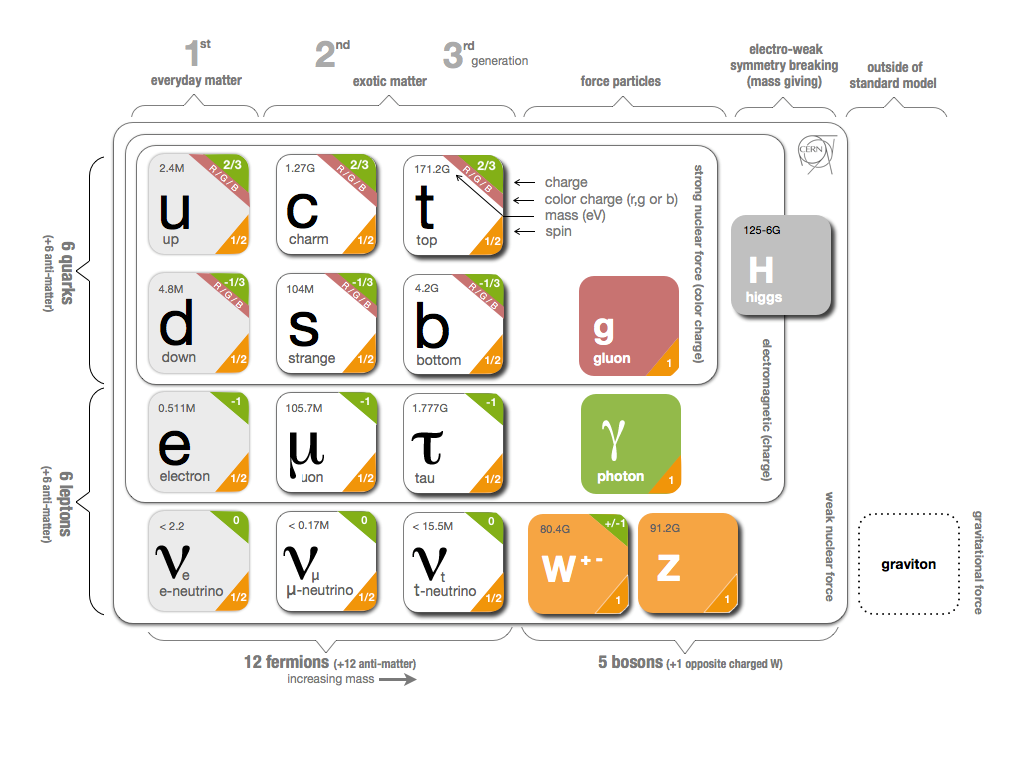
\includegraphics[width=0.9\textwidth]{pics/Intro/standard_model_cern.png}
    \caption{The Standard Model of particles physics: 12 elementary fermions and 5 elementary bosons.
             Plot taken from~\cite{SM_table_CERN}. }
    \label{fig:SM_table}
\end{figure*}

The theory of the SM is formulated in quantum field theory and exhibits rich physics phenomena.
The mathematical construction of the SM is given in the following sections:
Section~\ref{sec:gauge_symmetry} describes the basic formalism of quantum field theory and the idea of gauge symmetry;
Section~\ref{sec:SM_Lagrangian} shows the mathematical description of the SM without the Higgs field and its drawback in describing particle masses;
Section~\ref{sec:Higgs_mech} introduces the Higgs field and its interplay with the gauge fields and fermion fields which allows particles to retain masses;
and Section~\ref{sec:SM_parameters} discusses the free parameters in the SM and the motivation to study the Higgs to muons decay.


\section{Quantum field theory and gauge symmetry}\label{sec:gauge_symmetry}

Symmetry is a key concept in physics. 
A symmetry regarding a certain quantity means the equations of motion do not depend on this quantity
and implies the existence of a conservation law.
For example the symmetries under translations in space and time correspond to the conservations of momenta and energy.

In quantum field theory, the Lagrangian for a free Dirac field is 
\begin{equation}\label{eq:Dirac_Lagrangian}
    \mathcal{L} = \bar{\psi}(x)(i\gamma^{\mu}\partial_{\mu}-m)\psi(x)
\end{equation}
where $\psi(x)$ is the Dirac field,
$\partial_{\mu}$ is the regular partial derivative with Lorentz index $\mu$,
and $m$ is the mass of the Dirac spinor.
$\gamma_{\mu}$ denotes the Dirac matrices
\begin{equation}\label{eq:dirac_matrices}
    \gamma^{0} = \begin{pmatrix}  I_{2} & 0 \\ 0 & -I_{2}    \end{pmatrix} ~,~
    \gamma^{k} = \begin{pmatrix}  0 & \sigma^{k} \\ -\sigma^{k} & 0 \end{pmatrix} ~,~
    \text{with} ~ k = 1,2,3 
\end{equation}
where $I_{2}$ is the $2 \times 2$ identity matrix and $\sigma^{k}$ denotes the Pauli matrices.
\begin{equation}\label{eq:pauli_matrices}
    \sigma_{1} = \begin{pmatrix} 0 & 1 \\ 1 & 0 \end{pmatrix} ~,~
    \sigma_{2} = \begin{pmatrix} 0 & -i \\ i & 0\end{pmatrix} ~,~
    \sigma_{3} = \begin{pmatrix} 1 & 0 \\ 0 & -1\end{pmatrix}
\end{equation}

This Lagrangian is invariant under an internal phase translation
\begin{equation}\label{eq:global_phase}
    \psi(x) \to e^{i\theta_{0}}\psi(x)
\end{equation}
where $\theta_{0}$ is an arbitrary constant.
This is a global symmetry as $\theta_{0}$ is independent from the spacetime location.
A crucial practice in quantum field theory is to promote global symmetries to local symmetries, 
also known as gauge symmetries, under transformations like
\begin{equation}\label{eq:local_phase}
 \psi(x) \to e^{i\theta(x)}\psi(x)
\end{equation}
where $\theta(x)$ is no longer constant but a function of the spacetime coordinates~$x$.
Obviously Equation~\ref{eq:Dirac_Lagrangian} is not invariant under this gauge transformation, 
as the transformation give rise to a new term $\partial_{\mu}\theta(x)$.
The way to achieve gauge invariance is to replace the partial derivative $\partial_{\mu}$ by the covariant derivative, 
through whose construction new interactions are introduced.

The covariant derivative of transformation Equation~\ref{eq:local_phase} is written as
\begin{equation}\label{eq:cov_de_phase}
    D_{\mu} = \partial_{\mu} + \text{i}eA_{\mu}
\end{equation}
where $e$ is an arbitrary constant and $A_{\mu}$ is a new field whose behavior under the same transformation is
\begin{equation}\label{eq:EM_transformation}
    A_{\mu}(x) \to A_{\mu}(x) - \frac{1}{e}\partial_{\mu}\theta(x)
\end{equation}
In fact, this exact formula can be used to describe electromagnetism, 
for which $A_{\mu}$ is the vector potential of the electromagnetic field and $e$ is the electric charge.

Modifying Equation~\ref{eq:Dirac_Lagrangian} with Equation~\ref{eq:cov_de_phase} and adding the EM field term, 
we get a gauge invariant Lagrangian describing a Dirac field interacting with an EM field
\begin{equation}\label{eq:Dirac_EM}
    \mathcal{L} = \bar{\psi}(x)(i\gamma^{\mu}D_{\mu}-m)\psi(x) - \frac{1}{4}F_{\mu\nu}F^{\mu\nu}
\end{equation}
where $F_{\mu\nu}$ is the EM field tensor
\begin{equation}\label{eq:EM_tensor}
    F_{\mu\nu}(x) = \partial_{\mu}A_{\nu}(x) - \partial_{\nu}A_{\mu}(x) 
\end{equation}
The transformation Equation~\ref{eq:local_phase} takes the form of the group U(1) at each point $x$.
Therefore we say the electromagnetic interaction follows a U(1) gauge symmetry.



\section{The standard model Lagrangian}\label{sec:SM_Lagrangian}

Following the formalism in Section~\ref{sec:gauge_symmetry} and knowing there are 6 quarks, 6 leptons, and 4 gauge bosons,
the SM Lagrangian without considering a Higgs boson and without mass terms can be written as:
\begin{equation}\label{eq:SM_Lagrangian}
  \begin{split}
    \mathcal{L} = & \bar{\psi}^{i} (i\gamma^{\mu})(D_{\mu})_{ij}\psi^{j} -
                  - \frac{1}{4} G^{k}_{\mu\nu}G^{k\mu\nu}
                  - \frac{1}{4} W^{a}_{\mu\nu}W^{a\mu\nu}
                  - \frac{1}{4} B_{\mu\nu}B^{\mu\nu}
  \end{split}
\end{equation}
In the equation:
\begin{itemize}
  \item $\psi$ is the fermion field and $D_{\mu}$ is the covariant derivative;
  \item $G^{k}_{\mu\nu}$, $W^{a}_{\mu\nu}$, and $B_{\mu\nu}$ are field strength tensors for the interaction fields 
        corresponding to the groups SU(3), an SU(2), and an U(1), respectively;
  \item $\mu$ and $\nu$ are the Lorentz vector indices. Index $k$ and $a$ are the index of the group generators, $k$ running from 1 to 8, and $a$ running from 1 to 3;
\end{itemize}


This Lagrangian takes the structure of groups SU$(3)_{c} \times$SU$(2)_{L} \times$U$(1)_{Y}$.
The SU$(3)_{c}$ represents the strong interaction with the subscript $c$ standing for color.
The SU$(2)_{L} \times$U$(1)_{Y}$ is the electroweak interaction, 
where the $L$ means it only acts on left-handed fermions
and the $Y$ is the hypercharge associated with the U(1) group.\footnote{The hypercharge $Y$ is not the electric charge $e$ in Equation~\ref{eq:cov_de_phase}.
In fact, for all fermions, the electric charge $Q = T_{3} + Y/2$.}
Here the SU$(2)_{L} \times$U$(1)_{Y}$ cannot be disentangled and viewed separately as the weak interaction and electromagnetic interaction.

The gauge transformations on the fermion field are:
\begin{equation}\label{eq:gauge_fermion}
  \begin{split}
    \text{U(1)}:  & ~~~~ \psi(x) \to  \text{exp}[i\theta_{Y}(x)Y]\psi(x) \\
    \text{SU(2)}: & ~~~~ \psi(x) \to  \text{exp}[i\theta^{a}_{L}(x)T^{a}]\psi(x) \\
    \text{SU(3)}: & ~~~~ \psi(x) \to  \text{exp}[i\theta^{k}_{c}(x)t^{k}]\psi(x) 
  \end{split}  
\end{equation}  
with $D_{\mu}$ taking the form of 
\begin{equation}\label{eq:SM_cov_dev}
  D_{\mu} = \partial_{\mu} - ig^{\prime}B_{\mu}Y - igW^{a}_{\mu}T^{a} - ig_{s}G^{k}_{\mu}t^{k}
\end{equation} 
where $g^{\prime}$, $g$, and $g_{s}$ are field strength coefficients, 
and $Y$, $T^{a}$, and $t^{k}$ are interaction operators, for U(1), SU(2), and SU(3) respectively.
In this construction the transformations on the interaction fields are:
\begin{equation}\label{eq:gauge_interaction}
  \begin{split}
    \text{U(1)}:  & ~~~~  B_{\mu}(x) \to B_{\mu}(x) + \frac{1}{g^{\prime}}\partial_{\mu}\theta_{Y}(x) \\
    \text{SU(2)}: & ~~~~  W^{a}_{\mu}(x) \to  W^{a}_{\mu}(x) + \frac{1}{g}\partial_{\mu}\theta^{a}_{L}(x) + \epsilon^{abc}W^{b}_{\mu}(x)\theta^{c}_{L}(x) \\
    \text{SU(3)}: & ~~~~  G^{k}_{\mu}(x) \to  G^{k}_{\mu}(x) + \frac{1}{g_{s}}\partial_{\mu}\theta^{k}_{c}(x) + f^{klm}G^{l}_{\mu}(x)\theta^{m}_{c}(x)
  \end{split}  
\end{equation}  
Furthermore, the field tensors in Equation~\ref{eq:SM_Lagrangian} are related to the field vectors as
\begin{equation}\label{eq:field_tensor}
  \begin{split}
    \text{U(1)}:  & ~~~~ B_{\mu\nu} = \partial_{\mu}B_{\nu} - \partial_{\nu}B_{\mu} \\
    \text{SU(2)}: & ~~~~ W^{a}_{\mu\nu} = \partial_{\mu}W^{a}_{\nu} - \partial_{\nu}W^{a}_{\mu} + g\epsilon^{abc}W^{b}_{\mu}W^{c}_{\nu} \\
    \text{SU(3)}: & ~~~~ G^{k}_{\mu\nu} = \partial_{\mu}G^{k}_{\nu} - \partial_{\nu}G^{k}_{\mu} + g_{s} f^{klm}G^{l}_{\mu}G^{m}_{\mu} 
  \end{split}
\end{equation}
in which the $\epsilon^{abc}$ and $f^{klm}$ are structure constants of SU(2) and SU(3) governing the relations between group generators
\begin{equation}\label{eq:struture_constant}
  \begin{split}
    [T^{a}, T^{b}] = i\epsilon^{abc}T_{c} \\
    [t^{k}, t^{l}] = if^{klm}t_{m}
  \end{split}
\end{equation}


Equation~\ref{eq:SM_Lagrangian} models the strong and electroweak interactions with matter fields.
However, all particles in this model are massless as there are no mass terms like
\begin{equation}\label{eq:mass_Lagrangian}
    \mathcal{L}_{\text{mass}} = - m_{f} \bar{\psi}^{i}_{f} \psi_{fi}
                                + \frac{1}{2} m^{2}_{G} G_{\mu}G^{\mu}
                                + \frac{1}{2} m^{2}_{W} W_{\mu}W^{\mu}
                                + \frac{1}{2} m^{2}_{B} B_{\mu}B^{\mu}
\end{equation}
None of these terms is gauge invariant.
The gauge boson terms, $m^{2}_{G} G_{\mu}G^{\mu}$, $m^{2}_{W} W_{\mu}W^{\mu}$, and $m^{2}_{B} B_{\mu}B^{\mu}$,
are not gauge invariant because their transformations always introduce new terms depending on the transformations as described in Equation~\ref{eq:gauge_interaction}. 
The reason why the fermion terms, $m_{f} \bar{\psi}^{i}_{f} \psi_{fi}$, are not gauge invariant is not so obvious in this form 
but becomes clear when written in left and right chiral forms: $\psi = \psi_{R} + \psi_{L}$,
in which 
\begin{equation}\label{eq:psi_chiral}
    \psi_{R} = \begin{pmatrix} \psi_{+} \\ 0 \end{pmatrix}, 
    ~\text{and}~
    \psi_{L} = \begin{pmatrix} 0 \\ \psi_{-} \end{pmatrix}
\end{equation}
We also introduce the projection operators:
\begin{equation}\label{eq:projection_op}
    P_{\pm} = \frac{1}{2}(1 \pm \gamma^{5}), ~\text{with}~ \gamma^{5} = i\gamma^{0}\gamma^{1}\gamma^{2}\gamma^{3}
\end{equation}
who act on $\psi$ as
\begin{equation}\label{eq:proj_psi}
  \begin{split}
    P_{+}\psi = \psi_{R}, & ~~~ P_{-}\psi = \psi_{L}, \\
    \bar{\psi}P_{+} = \bar{\psi_{L}}, & ~~~ \bar{\psi}P_{-} = \bar{\psi_{R}}
  \end{split}
\end{equation}
Expanding the term $m\bar{\psi} \psi = m(\bar{\psi_{R}} + \bar{\psi_{L}}) (\psi_{R} + \psi_{L})$,
the terms $\bar{\psi_{R}}\psi_{R}$ and $\bar{\psi_{L}}\psi_{L}$ vanish.
\begin{equation}\label{eq:RR_term}
    \bar{\psi_{R}}\psi_{R} = \bar{\psi} P_{-}P_{+} \psi = \bar{\psi} \frac{1}{4} (1 - (\gamma^{5})^{2}) \psi = 0
\end{equation}
The surviving terms are $m\bar{\psi} \psi = m\bar{\psi_{R}}\psi_{L} + m\bar{\psi_{L}}\psi_{R}$.
The SU$(2)_{L}$ transformation only acts on the left chiral component,
so its phase only appear in $\psi_{L}$ and is not canceled by $\psi_{R}$.
The U$(1)_{Y}$ hypercharge is also different for the left and right components,
leaving the U(1) phase uncanceled.
Therefore the fermion mass terms are not gauge invariant.\footnote{The surviving terms of $\bar{\psi} (i\gamma^{\mu})(D_{\mu})\psi$
are $\bar{\psi_{R}} (i\gamma^{\mu})(D_{\mu})\psi_{R}$ and $\bar{\psi_{L}} (i\gamma^{\mu})(D_{\mu})\psi_{L}$, 
in which the SU$(2)_{L}$ "phase" term cancels properly, making them gauge invariant.}

Therefore, Equation~\ref{eq:mass_Lagrangian} cannot be attached to Equation~\ref{eq:SM_Lagrangian} and all particles must be massless,
which contradicts the experimental findings.
The follow section describes a mechanism to allow particles to retain masses 
through the introduction of a new field component called the Higgs field.


\section{The Higgs mechanism}\label{sec:Higgs_mech}

The Higgs field is a complex scalar field whose potential is:
\begin{equation} \label{eq:Higgs_potential}
    V(\Phi) = - \mu^{2} \Phi^{\dagger}\Phi + \lambda(\Phi^{\dagger}\Phi)^{2}
\end{equation}
in which $\Phi$ is the complex scalar field and $\mu$, $\lambda$ are coefficients.
The shape of the this potential is shown in Figure~\ref{fig:Higgs_potential}. 
Parameter $\lambda$ needs to be positive for $V(\Phi)$ to have a minimum (ground state).
If $\mu^{2} \leqslant 0$, there is a single minimum of $V(\Phi)$ at zero when $|\Phi| = 0$.
If $\mu^{2} > 0$, $V(\Phi)$ can have a degenerate minimum of $-\frac{\mu^{4}}{4\lambda}$ when $\Phi^{\dagger}\Phi = \frac{\mu^{2}}{2\lambda}$.

\begin{figure*}[!htb]
  \centering
  \captionsetup{justification=justified}
  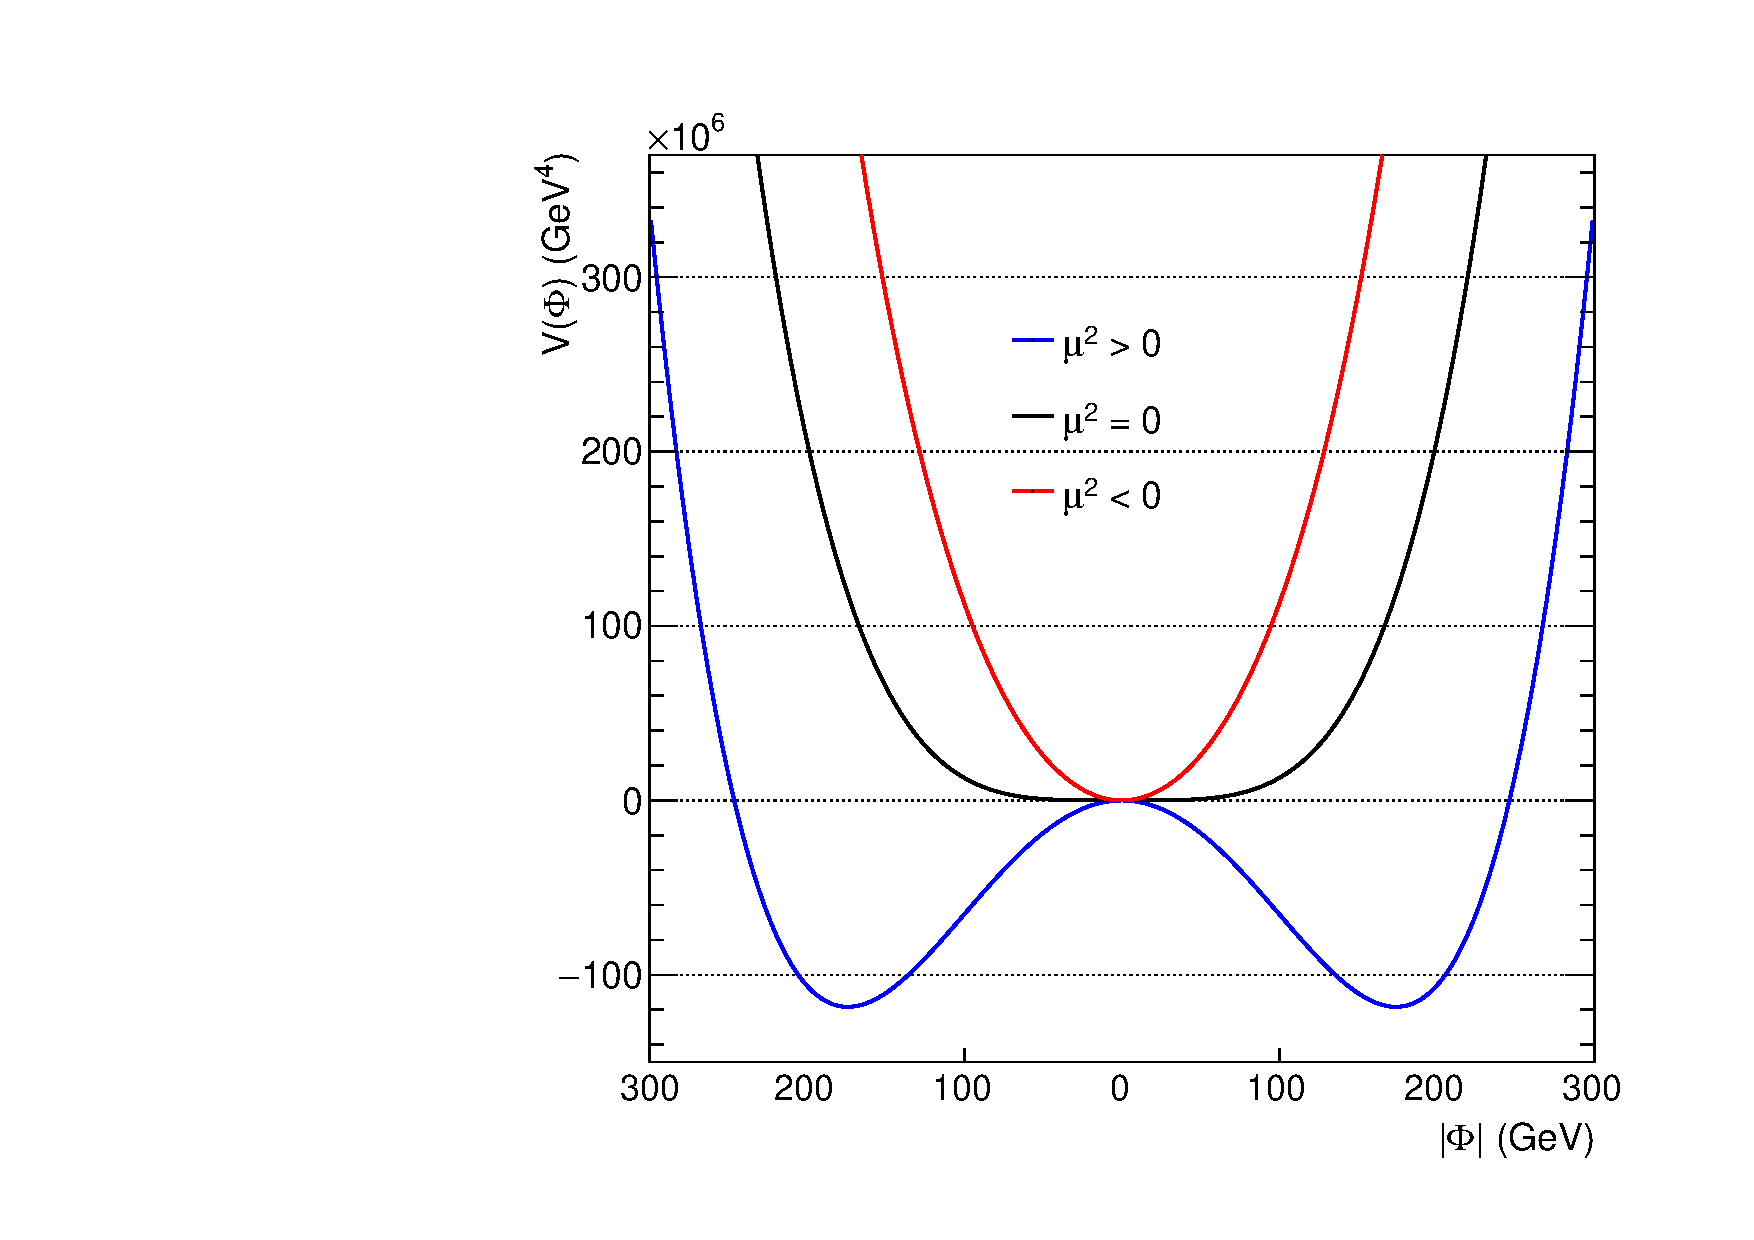
\includegraphics[width=0.6\textwidth]{pics/Intro/Higgs_field.pdf}
  \caption{The shape of the Higgs potential with different $\mu^{2}$ parameter configurations.}
  \label{fig:Higgs_potential}
\end{figure*}

The equation $\Phi^{\dagger}\Phi = \frac{\mu^{2}}{2\lambda}$ represents a circle in the complex plane of $\Phi$.
As $\mu^{2}$ increase from below 0 to above 0, 
the ground state of the field moves from $\Phi = 0$ in an arbitrary direction to a point on the circle $\Phi^{\dagger}\Phi = \frac{\mu^{2}}{2\lambda}$, 
making an asymmetric solution.
This phenomenon is known as the spontaneous symmetry breaking, 
which is also widely observed in physics systems such as the 
bending of a cylindrical rod under axial pressure,
or the cooling of a ferromagnetic material across its Curie temperature.

% Writing the Higgs field together with the simplest gauge field $A_{\mu}$, the Lagrangian is 
% \begin{equation}\label{eq:Higgs_gauge_Lag}
%   \mathcal{L} = |(\partial_{\mu}+ieA_{\mu})\Phi|^{2} -\frac{1}{4}F_{\mu\nu}F^{\mu\nu} + \mu^{2} \Phi^{\dagger}\Phi - \lambda(\Phi^{\dagger}\Phi)^{2}
% \end{equation}
% This Lagrangian itself is invariant under the U(1) gauge symmetry
% \begin{equation}\label{eq:U1_trans}
%     \Phi \to \text{exp}[i\theta(x)]\Phi, ~~~ A_{\mu} \to A_{\mu} - \frac{1}{e} \partial_{\mu}\theta(x)  
% \end{equation}
% but the symmetry breaks as the Higgs field takes a nonzero ground state.
% The fields can be rewritten as
% \begin{equation}\label{eq:Higgs_perturb_form}
%     \Phi(x) \to \frac{1}{\sqrt{2}} (\rho(x)+v)\text{exp}[i\zeta(x)/v], ~~~~~
%     A_{\mu} \to A_{\mu} - \frac{1}{ev} \partial_{\mu}\zeta(x)
% \end{equation}
% where $v = \frac{\mu^{2}}{\lambda}$ is known as the vacuum expectation value,
% $\rho(x)$ and $\zeta(x)$ are scale and phase deviations from this ground state position.
% The Lagrangian now becomes 
% \begin{equation}\label{eq:local_Higgs_gauge_Lag}
%   \begin{split}
%     \mathcal{L} = & -\frac{1}{4}F_{\mu\nu}F^{\mu\nu} + \frac{1}{2} e^{2}v^{2}A_{\mu}A^{\mu} 
%                     + e^{2}v \rho A_{\mu}A^{\mu} + \frac{1}{2} e^{2}\rho^{2}A_{\mu}A^{\mu} \\
%                   & + \frac{1}{2} |\partial_{\mu}\rho|^{2} + \lambda v^{2} \rho^{2} 
%                     - \lambda v \rho^{3} - \frac{1}{4} \lambda \rho^{4} + \frac{1}{4} \lambda v^{4}   
%   \end{split}
% \end{equation}
% In this Lagrangian, a massive gauge boson term $e^{2}v^{2}A_{\mu}A^{\mu}$ appears,
% and the $\rho$ becomes the apparent Higgs field.
% This is a simple example but it already shows rich physics content:
% it describes the coupling between the Higgs boson and the gauge boson $\rho A_{\mu}A^{\mu}$,
% and the 4-point coupling $\rho^{2}A_{\mu}A^{\mu}$,
% as well as the triple and quartic Higgs self-couplings, $\rho^{3}$ and $\rho^{4}$.


Now we look at the SM Lagrangian.
Putting the massless form of Equation~\ref{eq:SM_Lagrangian} together with the Higgs field, it becomes:
\begin{equation}\label{eq:SM_Lagrangian_Higgs}
  \begin{split}
    \mathcal{L} = &  - \frac{1}{4} G^{a}_{\mu\nu}G^{a\mu\nu}
                     - \frac{1}{4} W^{a}_{\mu\nu}W^{a\mu\nu}
                     - \frac{1}{4} B_{\mu\nu}B^{\mu\nu} \\
                  & + |D_{\mu}\Phi|^2 + \mu^{2} \Phi^{\dagger}\Phi - \lambda (\Phi^{\dagger}\Phi)^{2} \\
                  & + \sum_{f} [\bar{\psi}^{f}_{R} (i\gamma^{\mu})(D_{\mu})\psi^{f}_{R} + \bar{\psi}^{f}_{L} (i\gamma^{\mu})(D_{\mu})\psi^{f}_{L}] \\
                  & - \sum_{f} g_{f} [\bar{\psi}^{f}_{R}\Phi^{\dagger}\psi^{f}_{L} + \bar{\psi}^{f}_{L}\Phi\psi^{f}_{R} + \bar{\psi}^{f}_{R}\tilde{\Phi}^{\dagger}\psi^{f}_{L} + \bar{\psi}^{f}_{L}\tilde{\Phi}\psi^{f}_{R}]
  \end{split} 
\end{equation}
where the first and second lines are the gauge field and Higgs field,
the third line is the fermion kinetics written in the chiral form,
and the fourth line is the Yukawa coupling between fermions and the Higgs, also in the chiral form.
The index $f$ in the third and fourth lines just sums all fermions, 
with $g_{f}$ as the coupling strength for each fermion type.
The $\psi_{L}$ are doublets of the SU(2)
\begin{equation}\label{eq:SU2_doublet}
    \psi_{L} = \frac{1}{2} (1+\gamma_{5}) \begin{pmatrix} \nu^{i} \\ l^{i} \end{pmatrix},
    ~~~\text{or}~~~
    \frac{1}{2} (1+\gamma_5) \begin{pmatrix} U^{i} \\ D^{i} \end{pmatrix}
\end{equation}
and $\psi_{R}$ are singlets
\begin{equation}\label{eq:SU2_singlet}
    \psi_{R} =  \frac{1}{2} (1-\gamma_{5}) l^{i}, ~~\frac{1}{2} (1-\gamma_{5}) U^{i}, ~~\text{or}~~\frac{1}{2} (1-\gamma_{5}) D^{i}
\end{equation}
where $\nu^{i}, l^{i}, U^{i}, D^{i}$ are neutrinos, charged leptons, up-type quarks and down-type quarks of three generations.
The existence of right-handed neutrinos is not confirmed by experiments and therefore not assumed in the (simplest) SM.  
The Higgs field is a doublet with 4 total degrees of freedom
\begin{equation}\label{eq:SU2_higgs}
    \Phi = \begin{pmatrix} \Phi^{+} \\ \Phi^{0} \end{pmatrix} 
         = \frac{1}{\sqrt{2}} ~ \begin{pmatrix} \phi^{1}+i\phi^{2} \\ \phi^{3}+i\phi^{4} \end{pmatrix}
    ~,~~
    \tilde{\Phi} = \begin{pmatrix} \Phi^{0\dagger} \\ -\Phi^{-} \end{pmatrix} 
                 = \frac{1}{\sqrt{2}} ~ \begin{pmatrix} \phi^{3}-i\phi^{4} \\ -\phi^{1}+i\phi^{2} \end{pmatrix}     
\end{equation}
By choosing the direction of symmetry breaking to be the real part of $\Phi^{0}$, 
we can make $\phi^{1} = \phi^{2} = \phi^{4} = 0$ at the ground state,
and rewrite the Higgs doublet as
\begin{equation}\label{eq:Higgs_ground}
    \Phi \to \frac{1}{\sqrt{2}} ~\text{exp}[i\theta^{a}_{L}(x)T^{a}] ~\text{exp}[i\theta_{Y}(x)Y] ~\begin{pmatrix} 0 \\ v + \rho \end{pmatrix}
\end{equation} 
with $v = \sqrt{\frac{\mu^{2}}{\lambda}}$ known as the vacuum expectation value,
and $\rho$ as the deviation from the ground state position.


\textbf{Mass of the Higgs boson} comes from the potential term $\mu^{2} \Phi^{\dagger}\Phi - \lambda (\Phi^{\dagger}\Phi)^{2}$,
which expands to 
\begin{equation}\label{eq:potential_expand}
  \mu^{2} \Phi^{\dagger}\Phi - \lambda (\Phi^{\dagger}\Phi)^{2}
  = \lambda v^{2} \rho^{2} - \lambda v \rho^{3} - \frac{1}{4} \lambda \rho^{4} + \frac{1}{4} \lambda v^{4}
\end{equation}
The perturbation $\rho$ acts as the apparent Higgs field.
The term $\lambda v^{2} \rho^{2}$ describes the Higgs mass
\begin{equation}\label{eq:Higgs_mass}
    m_{H} = \sqrt{2\lambda} v
\end{equation}
Furthermore, terms $\rho^{3}$ and $\rho^{4}$ describes important Higgs properties of the triple and quartic self-couplings.

\textbf{Masses of gauge bosons} come from the $|D_{\mu}\Phi|^2$ term, which expands to
\begin{equation}\label{eq:gauge_mass_term}
  \begin{split}
    |D_{\mu}\Phi|^{2} = & \frac{1}{2}|\partial_{\mu}\rho|^{2} 
                        + \frac{1}{8}(v+\rho)^{2} [g^{2}(W^{1}_{\mu}W^{1\mu} + W^{2}_{\mu}W^{2\mu}) + (g^{\prime}B_{\mu}-gW^{3}_{\mu})^{2}] \\
                      = & \frac{1}{8}v^{2} [2g^{2}W^{+}_{\mu}W^{-\mu} + (g^{2}+g^{\prime 2})Z_{\mu}Z^{\mu}] \\
                        & + \frac{1}{4}v\rho [2g^{2}W^{+}_{\mu}W^{-\mu} + (g^{2}+g^{\prime 2})Z_{\mu}Z^{\mu}] \\
                        & + \frac{1}{8}\rho^{2} [2g^{2}W^{+}_{\mu}W^{-\mu} + (g^{2}+g^{\prime 2})Z_{\mu}Z^{\mu}] + \frac{1}{2}|\partial_{\mu}\rho|^{2}
  \end{split}
\end{equation}
In the second step the mass eigenstates of gauge bosons are defined as  
\begin{equation}\label{eq:V_boson_def}
  \begin{split}
    W^{\pm}_{\mu} & = \frac{W^{1}_{\mu} \mp iW^{2}_{\mu}}{\sqrt{2}} \\
    Z_{\mu} & = -\text{sin}\theta_{W} B_{\mu} + \text{cos}\theta_{W} W^{3}_{\mu} \\
    A_{\mu} & = \text{cos}\theta_{W} B_{\mu} + \text{sin}\theta_{W} W^{3}_{\mu}
  \end{split}
\end{equation}
with the Weinberg angle tan$\theta_{W} = g^{\prime}/g$.
The first part in Equation~\ref{eq:gauge_mass_term} becomes the mass terms for the gauge bosons with
\begin{equation}\label{eq:gauge_mass}
  \begin{split}
    m_{W} & = \frac{vg}{2} \\
    m_{Z} & = \frac{v\sqrt{g^{2}+g^{\prime 2}}}{2} \\
    m_{A} & = 0
  \end{split}
\end{equation}
In addition, the second part of Equation~\ref{eq:gauge_mass_term} describes the 3-point couplings between a Higgs boson and a pair of gauge bosons,
while the third part describes the 4-point couplings between a Higgs boson pair and a gauge boson pair.

\textbf{Masses of fermions} come from the Yukawa coupling term in Equation~\ref{eq:SM_Lagrangian_Higgs}.
The term $\bar{\psi}^{f}_{R}\Phi^{\dagger}\psi^{f}_{L} + \bar{\psi}^{f}_{L}\Phi\psi^{f}_{R}$ gives the masses for charged leptons and down-type quarks.
\begin{equation}\label{eq:yukawa_mass}
  \begin{split}
      & -\sum_{f} g_{f} [\bar{\psi}^{f}_{R}\Phi^{\dagger}\psi^{f}_{L} + \bar{\psi}^{f}_{L}\Phi\psi^{f}_{R} ] \\
    = & - \sum_{l^{i}} g_{l^{i}} ~\frac{1}{2\sqrt{2}}~\bar{l}^{i} ~\begin{pmatrix} 0 ,& v+\rho \end{pmatrix} ~\begin{pmatrix} \nu^{i} \\ l^{i} \end{pmatrix}
        - \sum_{l^{i}} g_{l^{i}} ~\frac{1}{2\sqrt{2}}~\begin{pmatrix} \bar{\nu}^{i} ,& \bar{l}^{i} \end{pmatrix} ~\begin{pmatrix} 0 \\ v+\rho \end{pmatrix} ~l^{i} \\
      & - \sum_{D^{i}} g_{D^{i}} ~\frac{1}{2\sqrt{2}}~\bar{D}^{i} ~\begin{pmatrix} 0 ,& v+\rho \end{pmatrix} ~\begin{pmatrix} U^{i} \\ D^{i} \end{pmatrix}
        - \sum_{D^{i}} g_{D^{i}} ~\frac{1}{2\sqrt{2}}~\begin{pmatrix} \bar{U}^{i} ,& \bar{D}^{i} \end{pmatrix} ~\begin{pmatrix} 0 \\ v+\rho \end{pmatrix} ~D^{i} \\
    = & - \frac{1}{\sqrt{2}} \sum_{l^{i}} g_{l^{i}}  (v+\rho) \bar{l}^{i} l^{i}
        - \frac{1}{\sqrt{2}} \sum_{D^{i}} g_{D^{i}}  (v+\rho) \bar{D}^{i} D^{i}    
  \end{split}
\end{equation}
In this equation some calculations are omitted to save space:
the SU(2) phase cancels between $\Phi^{\dagger}$ and $\psi_{L}$, 
the SU(1) phase cancels between $\bar{\psi_{R}}$, $\Phi^{\dagger}$ and $\psi_{L}$ as their hypercharges add up to 0,
and the product of projection operators in $\bar{\psi}_{R}$ and $\psi_{L}$ is 2 and is absorbed in the coefficients.
Similar to Equation~\ref{eq:yukawa_mass}, the term $\bar{\psi}^{f}_{R}\tilde{\Phi}^{\dagger}\psi^{f}_{L} + \bar{\psi}^{f}_{L}\tilde{\Phi}\psi^{f}_{R}$ gives the masses for up-type quarks.
\begin{equation}
    - \sum_{f} g_{f} [\bar{\psi}^{f}_{R}\tilde{\Phi}^{\dagger}\psi^{f}_{L} + \bar{\psi}^{f}_{L}\tilde{\Phi}\psi^{f}_{R}]
    = - \frac{1}{\sqrt{2}} \sum_{U^{i}} g_{U^{i}}  (v+\rho) \bar{U}^{i} U^{i}
\end{equation}
There is no term here for neutrinos as they do not have right-handed components.
Overall, the Yukawa term is summarized as
\begin{equation}\label{eq:Lagrangian_yukawa}
    \mathcal{L}_{\text{Yukawa}} = - \sum_{f} \frac{1}{\sqrt{2}} g_{f} (v\bar{\psi}^{f}\psi^{f} + \rho \bar{\psi}^{f}\psi^{f})
\end{equation}
where the first part is the mass term for fermions, 
and the second part is the interactions between the apparent Higgs field $\rho$ and the fermions.
The fermion mass $m_{f}$ is proportional to its Yukawa coupling strength $g_{f}$
\begin{equation}\label{eq:fermion_mass}
    m_{f} = \frac{vg_{f}}{\sqrt{2}}
\end{equation} 


\section{Parameters of the standard model}\label{sec:SM_parameters}

In the Lagrangian we derived in the last Section, there are 14 unconstrained real parameters (assuming massless neutrinos):
\begin{itemize}
  \item 3 gauge coupling constants $g$, $g^{\prime}$, and $g_{s}$;
  \item 2 Higgs potential shape parameters $\lambda$ and $\mu^{2}$;
  \item 9 Yukawa coupling constants $g_{f}$ for 3 charged leptons and 6 quarks.
\end{itemize}
There are 5 other parameters not elaborated here
\begin{itemize}
  \item 4 parameters in the quark mixing matrix (CKM matrix) which is not elaborated here, including 3 angle parameters and 1 phase parameter;
  \item A parameter for CP violation in the strong interaction.
\end{itemize}
These total 19 parameters determine the exact properties of SM particles and the measurements of them are a key topic of high energy experiments. 
In practice, some other variable sets are frequently used. 
For example, the parameter set $[g, g^{\prime}, \lambda, \mu^{2}, g_{f}]$ is interchangeable with 
the set consisting of the vacuum expectation, and the masses of Higgs, \PW, \PZ, and fermions $[v, m_{H}, m_{W}, m_{Z}, m_{f}]$.


The Higgs boson was first observed at the LHC by ATLAS and CMS Collaborations in 2012~\cite{Aad:2012tfa, Chatrchyan:2012xdj, Chatrchyan:2013lba}.
Various measurements on the Higgs properties have been conducted to verify their agreement with the SM prediction and to put constraints on the free SM parameters.
The latest and most precise measurement of the Higgs mass is $125.38 \pm 0.14$ \GeV, provided by the CMS Collaboration~\cite{2020135425}. 
The Higgs decays to gauge bosons and third-generation fermions (except the top quark) have been observed 
and measured~\cite{Sirunyan:2312121, 201996, Sirunyan:2017exp, PhysRevLett.121.121801, 2018283, PhysRevD.99.072001, 201859, 2019508, Aaboud_2018}.
The Higgs coupling to the top quark has also been measured through the Higgs production process in association with a top quark pair~\cite{PhysRevLett.120.231801, 2018173}.
The Higgs coupling measurements from CMS with the LHC proton-proton collision data collected in 2016 is summarized in Figure~\ref{fig:higgs_2016},
in which, the gauge couplings and Yukawa couplings are expressed by the coupling modifiers 
($\kappa_{\PW}$, $\kappa_{\PZ}$, $\kappa_{t}$, $\kappa_{\tau}$, $\kappa_{b}$, and $\kappa_{\mu}$) in the \kappa-framework~\cite{Heinemeyer:2013tqa}.
This result confirms the proportionality between fermion masses and their coupling strengths to the Higgs boson,
a behavior predicted by the SM in Equation~\ref{eq:fermion_mass}.

The Higgs couplings to fermions of the first and second generations, 
however, are expected to be small and hard to probe.
The study of Higgs to muons decay is of particular importance 
as it is the most experimentally sensitive way to probe Higgs couplings to second-generation fermions.
 

%\begin{table}[!htb]
%  \centering
%  \captionsetup{justification=justified}
%  \topcaption{The branching fractions of the main decay modes of the SM Higgs boson with a mass of 125 \GeV.}
%  \begin{tabular}{lc}
%    \hline
%    Decay mode                 &  Branching fraction \\
%    \hline
%    $\PH \to \Pqb\Paqb$        &  58.4\% \\
%    $\PH \to \PW^{+}\PW^{-}$   &  21.4\% \\
%    $\PH \to gg$               &  8.19\% \\
%    $\PH \to \tau\bar{\tau}$   &  6.26\% \\
%    $\PH \to c\bar{c}$         &  2.89\% \\
%    $\PH \to \PZ\PZ$           &  2.62\% \\
%    $\PH \to \gamma\gamma$     &  0.227\% \\
%    $\PH \to \PZ\gamma$        &  0.153\% \\
%    $\PH \to \mu\bar{\mu}$     &  0.022\% \\
%    \hline
%  \end{tabular}
%  \label{tab:higgs_BR}
%\end{table}


\begin{figure*}[!htb]
    \centering
    \captionsetup{justification=justified}
    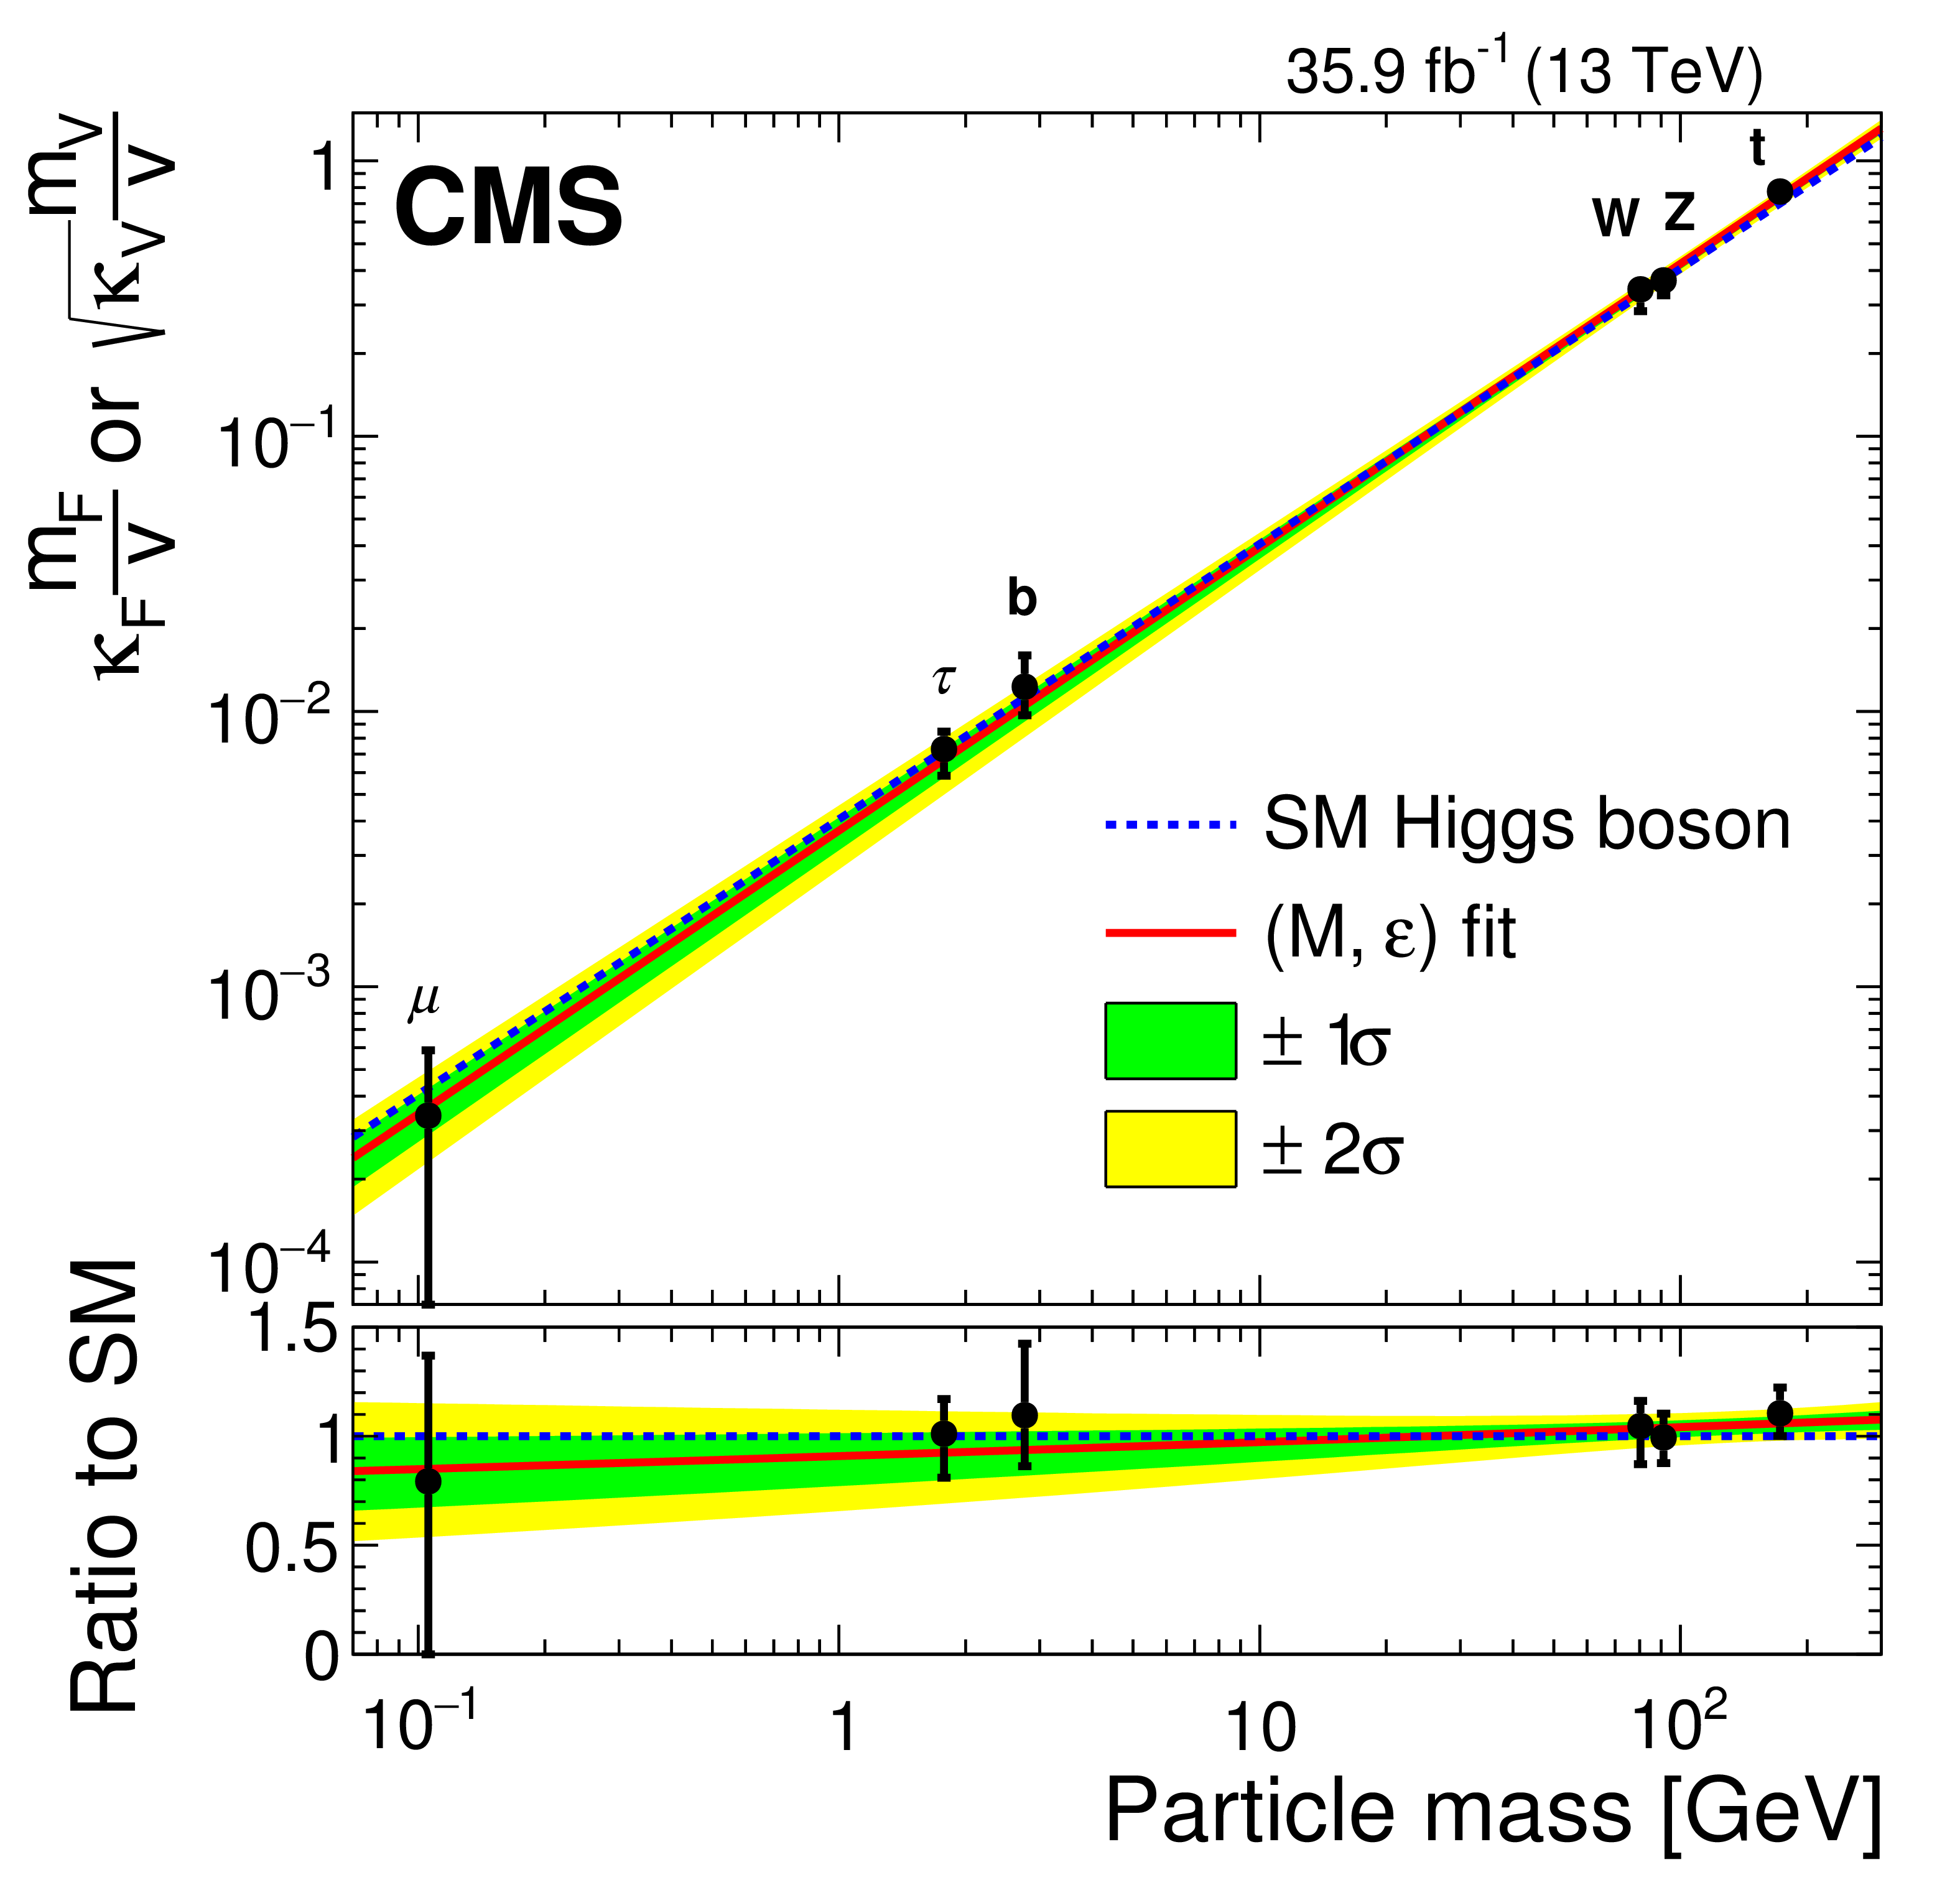
\includegraphics[width=0.60\textwidth]{pics/Intro/higgs_coupling_2016.png}
    \caption{Summary of the CMS measurements on the Higgs coupling to fermions and bosons.
             Plot taken from~\cite{Sirunyan:2640611}. }
    \label{fig:higgs_2016}
\end{figure*}


This thesis presents the recent analysis of the Higgs to muons decay from CMS 
with a focus on the work in the vector boson associated Higgs production channel (VH).
The following chapters are organized as follows:
Chapter~\ref{chp:LHC_CMS} describes the LHC machine and the CMS detector,
Chapter~\ref{chp:hmm_overview} gives an overview of the \hmm analysis 
which is conducted in 4 exclusive event categories targeting different Higgs production modes,
Chapter~\ref{chp:objects} lists the reconstruction of physics objects and the selections on them in the analysis,
Chapter~\ref{chp:muon_corr} details the correction methods and calibration studies on the muon momentum which is crucial to the accuracy of this work,
Chapter~\ref{chp:VH_analysis} reports the full procedures of the analysis in the VH channel,
and Chapter~\ref{chp:hmm_results} summarizes the results from the VH analysis 
as well as the combined results of all 4 analysis channels. 